\documentclass{article}
\usepackage{fontspec}
\setsansfont{Helvetica}
\renewcommand{\familydefault}{\sfdefault}
\usepackage{tikz}
\usetikzlibrary{arrows.meta}
\pagestyle{empty}
\definecolor{lookup}{HTML}{2A78D6}
\definecolor{lookuplight}{HTML}{9DC1EC}
\definecolor{write}{HTML}{EB6834}
\definecolor{writelight}{HTML}{F5B597}
\definecolor{ink}{HTML}{0B0B0B}
\definecolor{inktwo}{HTML}{52514E}
\definecolor{gridc}{HTML}{E4E3DF}
\definecolor{axisc}{HTML}{8F8E89}
\definecolor{refc}{HTML}{3D3C39}
\tikzset{
  tick/.style={font=\footnotesize, text=inktwo, inner sep=1.5pt},
  lab/.style={font=\small, text=ink, inner sep=1.5pt},
  note/.style={font=\footnotesize, text=inktwo, inner sep=1.5pt},
  ser/.style={line width=1.4pt, line cap=round, line join=round},
  thin/.style={line width=0.9pt, line cap=round, line join=round},
  ref/.style={line width=0.8pt, draw=refc, dash pattern=on 3pt off 2pt},
}
\begin{document}
\setbox0=\hbox{%
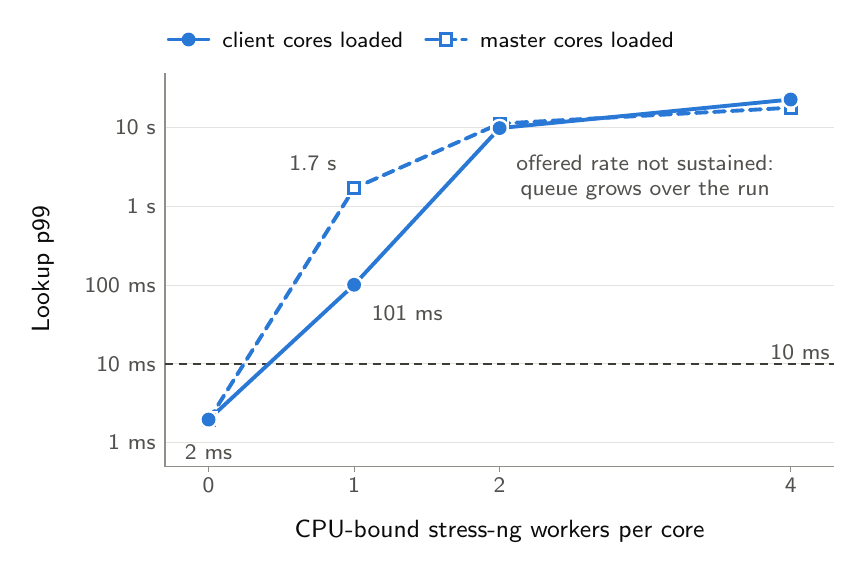
\begin{tikzpicture}[x=1cm,y=1cm]
\draw[draw=gridc, line width=0.4pt] (0.000,0.301) -- (8.500,0.301);
\node[tick, anchor=east] at (-0.060,0.301) {1 ms};
\draw[draw=gridc, line width=0.4pt] (0.000,1.301) -- (8.500,1.301);
\node[tick, anchor=east] at (-0.060,1.301) {10 ms};
\draw[draw=gridc, line width=0.4pt] (0.000,2.301) -- (8.500,2.301);
\node[tick, anchor=east] at (-0.060,2.301) {100 ms};
\draw[draw=gridc, line width=0.4pt] (0.000,3.301) -- (8.500,3.301);
\node[tick, anchor=east] at (-0.060,3.301) {1 s};
\draw[draw=gridc, line width=0.4pt] (0.000,4.301) -- (8.500,4.301);
\node[tick, anchor=east] at (-0.060,4.301) {10 s};
\draw[draw=axisc, line width=0.4pt] (0.554,0.000) -- (0.554,-0.070);
\node[tick, anchor=north] at (0.554,-0.090) {0};
\draw[draw=axisc, line width=0.4pt] (2.402,0.000) -- (2.402,-0.070);
\node[tick, anchor=north] at (2.402,-0.090) {1};
\draw[draw=axisc, line width=0.4pt] (4.250,0.000) -- (4.250,-0.070);
\node[tick, anchor=north] at (4.250,-0.090) {2};
\draw[draw=axisc, line width=0.4pt] (7.946,0.000) -- (7.946,-0.070);
\node[tick, anchor=north] at (7.946,-0.090) {4};
\draw[draw=axisc, line width=0.5pt] (0.000,5.000) -- (0.000,0.000) -- (8.500,0.000);
\draw[ref] (0.000,1.301) -- (8.500,1.301);
\draw[ser, draw=lookup, dash pattern=on 4pt off 2.5pt] (0.554,0.586) -- (2.402,3.531) -- (4.250,4.352) -- (7.946,4.554);
\draw[ser, draw=lookup] (0.554,0.593) -- (2.402,2.305) -- (4.250,4.295) -- (7.946,4.658);
\fill[white] (0.554,0.586) +(-3.3pt,-3.3pt) rectangle +(3.3pt,3.3pt);
\filldraw[fill=white, draw=lookup, line width=1.1pt] (0.554,0.586) +(-2.0pt,-2.0pt) rectangle +(2.0pt,2.0pt);
\fill[white] (2.402,3.531) +(-3.3pt,-3.3pt) rectangle +(3.3pt,3.3pt);
\filldraw[fill=white, draw=lookup, line width=1.1pt] (2.402,3.531) +(-2.0pt,-2.0pt) rectangle +(2.0pt,2.0pt);
\fill[white] (4.250,4.352) +(-3.3pt,-3.3pt) rectangle +(3.3pt,3.3pt);
\filldraw[fill=white, draw=lookup, line width=1.1pt] (4.250,4.352) +(-2.0pt,-2.0pt) rectangle +(2.0pt,2.0pt);
\fill[white] (7.946,4.554) +(-3.3pt,-3.3pt) rectangle +(3.3pt,3.3pt);
\filldraw[fill=white, draw=lookup, line width=1.1pt] (7.946,4.554) +(-2.0pt,-2.0pt) rectangle +(2.0pt,2.0pt);
\fill[white] (0.554,0.593) circle (3.4pt);
\fill[lookup] (0.554,0.593) circle (2.5pt);
\fill[white] (2.402,2.305) circle (3.4pt);
\fill[lookup] (2.402,2.305) circle (2.5pt);
\fill[white] (4.250,4.295) circle (3.4pt);
\fill[lookup] (4.250,4.295) circle (2.5pt);
\fill[white] (7.946,4.658) circle (3.4pt);
\fill[lookup] (7.946,4.658) circle (2.5pt);
\node[note, anchor=north] at (0.554,0.333) {2 ms};
\node[note, anchor=north west] at (2.402,2.097) {\;\;101 ms};
\node[note, anchor=south east] at (2.402,3.693) {1.7 s\;\;};
\node[note, anchor=south east] at (8.500,1.301) {10 ms};
\node[note, anchor=south] at (6.098,3.699) {offered rate not sustained:};
\node[note, anchor=north] at (6.098,3.699) {queue grows over the run};
\node[lab, anchor=north] at (4.250,-0.620) {CPU-bound stress-ng workers per core};
\node[lab, rotate=90, anchor=south] at (-1.350,2.500) {Lookup p99};
\draw[ser, draw=lookup] (0.050,5.420) -- (0.550,5.420);
\fill[lookup] (0.300,5.420) circle (2.5pt);
\node[note, anchor=west, text=ink] at (0.670,5.420) {client cores loaded};
\draw[ser, draw=lookup, dash pattern=on 4pt off 2.5pt] (3.320,5.420) -- (3.820,5.420);
\filldraw[fill=white, draw=lookup, line width=1.1pt] (3.570,5.420) +(-2.0pt,-2.0pt) rectangle +(2.0pt,2.0pt);
\node[note, anchor=west, text=ink] at (3.940,5.420) {master cores loaded};
\end{tikzpicture}}%
\pdfvariable horigin=0pt
\pdfvariable vorigin=0pt
\pagewidth=\dimexpr\wd0+8pt\relax
\pageheight=\dimexpr\ht0+\dp0+8pt\relax
\shipout\vbox{\kern4pt\hbox{\kern4pt\box0\kern4pt}\kern4pt}
\end{document}
